\documentclass[12pt]{book}
\usepackage[top=1in, bottom=1in, left=1.2in, right=1in, a4paper]{geometry}

 \ifx\pdftexversion\undefined
 \usepackage[dvips]{graphicx}
 \else
 
 \usepackage[pdftex]{graphicx}
 \DeclareGraphicsRule{*}{mps}{*}{}
 \fi
%\usepackage{tabularx,colortbl}
\usepackage{url}
\usepackage{chapterbib}
\usepackage{hyperref}
%\usepackage{tikz}
%\usepackage{pgfplots}
%\usepgfplotslibrary{groupplots} 
%\usepackage{pgf, pgfarrows, pgfnodes}
\usepackage{lscape}
\usepackage{longtable}
\usepackage{float}
\usepackage{url}
\usepackage{multicol}
\usepackage{color}

%\usepackage[none]{hyphenat}
\renewcommand{\bibname}{References}

\setcounter{secnumdepth}{4}
\setcounter{tocdepth}{4}

\begin{document}

\begin{titlepage}
 \begin{center}
\Huge
\textbf{IITB Summer Internship 2013} \\
\vfill

\includegraphics[width=3cm]{IITB_logo.png}
\vfill
\Huge
\textbf{Project Report}\\
\vfill
\textbf{Attachment for Aadhar Authentication on Aakash}\\
\vfill
\LARGE
\underline{\textbf{Principal Investigator}} \\
Prof. D.B. Phatak\\
\vfill
\LARGE
\underline{\textbf{Project In-Charge}} \\
Mr. Nagesh Karmali\\
\vfill
\Large

\begin{tabular}{l|l}
\textbf{Project Mentors} & \textbf{Project Team Members} \\
Miss. Birundha M. & Miss. Archana Iyer \\
Miss. Firuza Aibara (PMO) & Mr. Hitesh Yadav \\ 
Mr. Jugal Mehta & Miss. Pooja Deo \\
 & Mr. Prashant Main  \\
 & Mr. Prateek Somani  \\
 & Mr. Prathamesh Paleyekar \\
 & Miss. Sonu Philip \\
 & Mr. Sudhanshu Verma \\
\end{tabular}
\vfill

\includegraphics[width=2.0cm]{dj.jpg} \hfill

\includegraphics[width=2.0cm]{nitc.jpg} \hfill

\includegraphics[width=4.0cm]{t.jpg} \hfill

\includegraphics[width=2.0cm]{111.jpg} \hfill

\includegraphics[width=2.0cm]{vnit.jpg}
\vfill
Last Updated: \today
\end{center}
\end{titlepage}

 \pagebreak \textcolor{white}{text} \pagebreak
%\setcounter{page}{1}
%\pagenumbering{roman}
\thispagestyle{empty}

\begin{center}
\thispagestyle{empty}
\LARGE
\textbf{Summer Internship 2013 \\ Project Approval Certificate} \\
\vskip12pt
\Large
\textbf{Department of Computer Science and Engineering} \\
\vskip5pt
\textbf{Indian Institute of Technology Bombay} \\
\end{center}
\vfill
\normalsize
The project entitled ``Attachment for Aadhar Authentication on Aakash'' submitted by Miss. Archana Iyer, Mr. Hitesh Yadav, Miss. Pooja Deo, Mr. Prashant Main, Mr. Prateek Somani, Mr. Prathamesh Paleyekar, Miss. Sonu Philip and Mr. Sudhanshu Verma is approved for Summer Internship 2013 programme from 9th May 2013 to 6th July 2013, at Department of Computer Science and Engineering, IIT Bombay.

\vfill

\begin{multicols}{2}
\underline{\hspace{5cm}} \\
\indent Prof. Deepak B. Phatak \\
\indent Dept of CSE, IITB \\
\indent Principal Investigator \\

\begin{flushright}
\underline{\hspace{5cm}} \\
 Mr. Nagesh Karmali \\
\indent Dept of CSE, IITB \\
\indent Project In-charge \\
\end{flushright}
\end{multicols}

\vfill

\begin{center}
\underline{\hspace{5cm}} \\
 Mr. D. B. Sathe \\
 External Examiner \\
\end{center}
 
% \flushleft
 
 \vfill
Place:IIT Bombay, Mumbai\\

\intend Date:3rd July 2013 

 \pagebreak \thispagestyle{empty} \textcolor{white}{text} \pagebreak
 
\LARGE
\thispagestyle{empty}

\begin{center}
\textbf{Declaration}
\end{center}
\normalsize
I declare that this written submission represents my ideas in my own words and where 
others' ideas or words have been included, I have adequately cited and referenced the original 
sources.  I also declare that I have adhered to all principles of academic honesty and integrity 
and   have   not   misrepresented   or   fabricated   or   falsified   any   idea/data/fact/source   in   my 
submission.  I understand that any violation of the above will be cause for disciplinary action 
by the Institute and can also evoke  penal action from the sources which have thus not been 
properly cited or from whom proper permission has not been taken when needed.

\vfill
\begin{flushright}

\underline{\hspace{5cm}} \\
Miss. Archana Iyer \\
Dwarkadas J. Sanghvi College of Engineering \\

\vfill

\underline{\hspace{5cm}} \\
Mr. Hitesh Yadav \\ 
Visvesvaraya National Institute of Technology \\

\vfill

\underline{\hspace{5cm}} \\
Miss. Pooja Deo \\
Visvesvaraya National Institute of Technology\\

\vfill

\underline{\hspace{5cm}} \\
Mr. Prashant Main \\
Terna Engineering College \\

\vfill


\underline{\hspace{5cm}} \\
Mr. Prateek Somani \\
Bhagwan Mahavir College of Engineering and Technology \\

\vfill

\underline{\hspace{5cm}} \\
Mr. Prathamesh Paleyekar \\
Visvesvaraya National Institute of Technology \\

\vfill

\underline{\hspace{5cm}} \\
Miss. Sonu Philip \\
National Institute of Technology Calicut \\

\vfill

\underline{\hspace{5cm}} \\
Mr. Sudhanshu Verma \\
Visvesvaraya National Institute of Technology \\

\vfill
\end{flushright}
%\flushleft
\textbf{Date:} \underline{\hspace{5cm}}


\chapter*{Acknowledgment}
\setcounter{page}{1}
\pagenumbering{roman}
We would like to thank our guide, Prof. Deepak B Phatak for the consistent directions towards our work. Because of his consistent encouragement and right directions, we are able to do this project work.
We would also like to thank Mr Nagesh, our project in charge, for his constant support and suggestions throughout the making of this project, Miss Firuza Aibara for her insights into the different softwares used for the documentation and our mentors Mr Jugal and Miss Birundha for providing us with a systematic way for performing our project and helping us solve many problems we faced during the course of this project.
Finally we would also like to thank all the lab maintenance staff for providing us assistance in various h/w & s/w problems that we encountered during the course of our project.\\[12pt]
Participants

\chapter*{Abstract}
Aadhar authentication is the process wherein the Aadhar number, along with other attributes (demographic/biometrics/OTP) is submitted to UIDAI's Central Identities Data Repository (CIDR) for verification; the CIDR verifies whether the data submitted matches the data available in CIDR and responds with a “yes/no”. No personal identity information is returned as part of the response. The purpose of authentication is to enable residents to prove their identity and for service providers to confirm that the residents are ‘who they say they are' in order to supply services and give access to benefits.
The purpose of the project is to make an optical assembly for Aakash tablet so that it can be used in place of the current fingerprint scanning devices and to get a clear image of a fingerprint by using the tablet’s camera itself, and this fingerprint is in turn used for the authentication of the Aadhar Id, taking into consideration the cost of the optical device. Also an Image Enhancement Software is developed which will optimize the provided image. More specifically the system is designed in order to reduce the cost and to use the camera on the Aakash tablet for the purpose of fingerprint scanning. 
Once completed we will try for its application on other tablets and phones as well.

\listoffigures
%\listoftables
\tableofcontents

\pagebreak
\cleardoublepage

\setcounter{page}{1}
\pagenumbering{arabic}

\chapter{Introduction}

\section{Fingerprint Recognition System for Aadhar}

Aadhar “authentication” means the process wherein Aadhar Number, along with other attributes, including biometrics, are submitted to the Central Identities Data Repository (CIDR) for its verification on the basis of information or data or documents available with it.\\[12pt]
Aadhar authentication service only responds with a “yes/no” and no personal identity information is returned as part of the response.\\[12pt]
Authentication User Agency (AUA): An organization or an entity using Aadhar authentication as part of its applications to provide services to residents. Examples include Government Departments, Banks, and other public or private organizations. \\[12pt]
Sub-AUA (SA): An organization or a department or an entity having a business relationship with AUA offering specific services in a particular domain. \\[12pt]
Authentication requests emerging from an AUA contains the information on the specific SA. For example, a specific bank providing Aadhar enabled payment transaction through NPCI as the AUA becomes the SA. \\[12pt]
Authentication Service Agency (ASA): An organization or an entity providing secure leased line connectivity to UIDAI’s data centres for transmitting authentication requests from various AUAs.\\[12pt]
Terminal Devices: Terminal devices are devices employed by SAs/AUAs (both government and non-government) to provide services to the residents. \\[12pt]
Authentication Factors: \\[12pt]
Demographic data (name, address, date of birth etc.)\\
Biometric data (fingerprint image)\\
PIN\\
OTP\\
Possession of mobile\\

\begin{figure}[H]
 \centering
 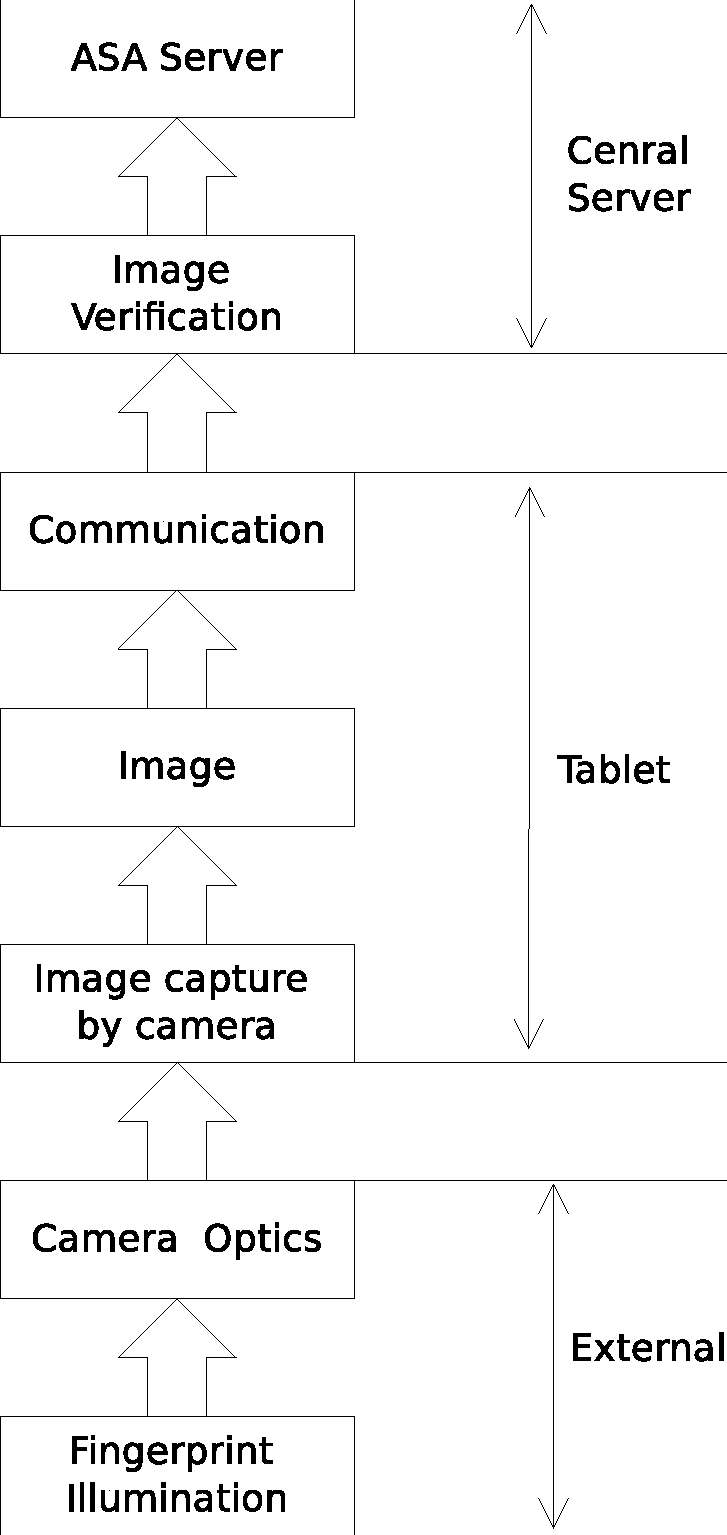
\includegraphics[width=7cm]{./Diagram1.pdf}
 \caption{Block diagram for Aadhar Authentication Process}
\end{figure}


\section{Aadhar Authentication}
Aadhar Number \\[12pt]
The Unique Identification (Aadhar) Number, which identifies a resident, will give individuals the means to clearly establish their identity to public and private agencies across the country. Three key characteristics of Aadhar Number are: \\[12pt]
1. Permanency (Aadhar number remains same during lifetime of a resident)\\[12pt]
2. Uniqueness (one resident has one ID and no two residents have same ID)\\[12pt]
3. Global (same identifier can be used across applications and domains)\\[12pt]
Aadhar Number is provided during the initiation process called enrolment where a resident’s demographic and biometric information are collected and uniqueness of the provided data is established through a process called de-duplication. \\[12pt]
Post reduplication, an Aadhar Number is issued and a letter is sent to resident informing the details.\\[12pt]

\section{Workflow of Aadhar authentication}
1. The hardware attached on the top of tablet’s camera takes the clear image for fingerprint authentication (biometric detail).	\\ [12pt]
2. Resident provides Aadhar Number, necessary demographic and biometric details to terminal devices belonging to the AUA/SA (or merchant/operator appointed by AUA/SA) to obtain a service offered by the AUA/SA. \\[12pt]
3. Aadhar authentication enabled application software that is installed on the device packages these input parameters, encrypts, and sends it to AUA server over either a mobile/broadband network using AUA specific protocol. \\[12pt]
4. AUA server, after validation adds necessary headers (AUA specific wrapper XML with license key, transaction id, etc.), and passes the request through ASA server to UIDAI CIDR. \\[12pt]
5. Aadhar authentication server returns a “yes/no” based on the match of the input parameters. \\[12pt] 
6. Based on the response from the Aadhar authentication server, AUA/SA conducts the transaction. \cite{abc} \\[12pt] \textcolor{white} {abc}


\chapter{Image Processing}

The steps involved in image processing are –\\[12pt]
1. Conversion of RGB to Gray scale \\[12pt]
2. Rescaling \\[12pt]
3. Adaptive Histogram equalization of Grey scale \\[12pt]
4. Sharpening \\ [12pt]
5. Thresholding\\[12pt]
6. Thinning\\[12pt]

\begin{figure}[H]
 \centering
 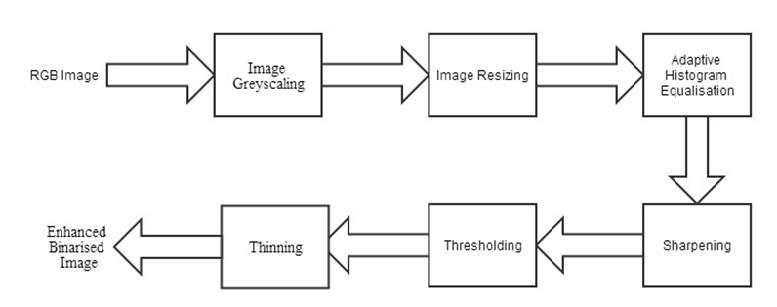
\includegraphics[width=15cm]{./1.jpg}
 \caption{Image Enhancement Workflow}
\end{figure}



\section{Conversion of RGB to Gray scale}
(a) The R, G and B values for each pixel are obtained.\\
(b) The average of these three values is calculated.\\
(c) Each pixel is reassigned this average value. \\

\section{Rescaling}
It is a process of resizing of the image.\\

\section{Adaptive Histogram equalization of Grey scale}
Adaptive histogram equalization (AHE) is a computer image processing technique used to improve contrast in images. It differs from ordinary histogram equalization in the respect that the adaptive method 
computes several histograms, each corresponding to a distinct section of the image, and uses them to redistribute the lightness values of the image. It is therefore suitable for improving the local contrast of an image and bringing out more detail.


\section{Sharpening}
Sharpening an image means to make the differences between the neighboring pixels more noticeable. Sharpening brings out the details of an image.
Sharpening can be done by kernel based convolutions.\\[12pt]
In image processing a kernel, is a small matrix which is useful for blurring, sharpening, embossing, edge-detection, and more. 
A kernel is a 2D matrix of numbers that can be used as coefficients for numerical operations on pixels.  

\begin{figure}[H]
 \centering
 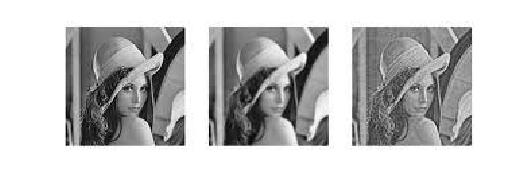
\includegraphics[width=10cm]{./9.jpg}
 \caption{Sharpened image}
\end{figure}
The third picture is a sharpened version of the original (first) image. \\[12pt]
Sharpening involves the following steps:\\[12pt]
1. Read the original image. \\
2. Choose the image processing technique-sharpening. \\
3. Choose the corresponding kernel to do the sharpening. \\
4. Apply the above kernel to the image matrix using convolution. \\
5. Display the sharpened image. \\[12pt]
The advantages of sharpening are that it brings out the details of an image, it makes the picture smudge free and it emphasizes on the texture of the image. \\[12pt]
The disadvantages of sharpening are that over-sharpening can spoil the originality of an image and by sharpening the smoothness of the image is lost. \\[12pt]
For sharpening one of the most commonly used methods is Laplacian kernel.\\[12pt]
The advantages of using laplacian kernel is that since the kernel is usually much smaller than the image, this method usually requires far fewer arithmetic operations and also, the Laplacian kernel is known in advance so only one convolution needs to be performed at run-time on the image.\\[12pt] 
The disadvantage of Laplacian kernel is that it is sensitive to noise.\\
To reduce the noise, the image is often Gaussian smoothed before applying the Laplacian filter.\\[12pt]
How convolution is done:\\[12pt]
\begin{figure}[H]
 \centering
 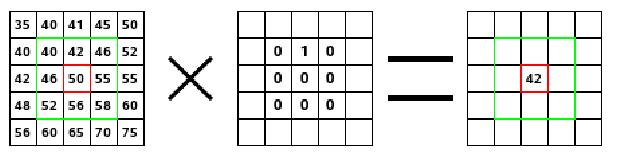
\includegraphics[width=10cm]{./3.jpg}
 \caption{Convolution technique}
\end{figure}
Complexity of Laplacian Kernel: \\[12pt]
Time Complexity=O(27 x m x n^2) \\[12pt]

m=size of the image\\[12pt]

n^2=multiplication complexity\\[12pt]

Space Complexity=O (m x 24)\\[12pt]

m=size of the image\\[12pt]

Another technique for doing sharpening is unsharp masking.\\[12pt]

The general algorithm is for unsharp masking is:\\[12pt] \\[12pt]
1. Blur the original. \\
2. Subtract the blurred image from the original (the resulting difference image is called the "mask"). \\
3. Amplify the difference.\\ 
4. Add the mask to the original. \\
5. The resulting image (original plus mask) will appear "sharper" \\[12pt]
Blurring can be done in different ways: \\
1. Using bilateral filter \\
2. Using median filter \\
3. Using mean filter \\[12pt]
The general algorithm is the same for all of the above techniques. \\
They vary in their method of blurring. \\[12pt]
The disadvantages of unsharp masking is that there are many steps and choices so the complexity is more. If we want to sharpen the edges then convolution is better since in unsharp masking everything is sharpened, not just the edges where sharpening is most needed. Also by doing unsharp masking the noise is amplified. One convolution has to be applied to blur the image. In unsharp masking the number of multiplication steps is more because there are more steps in unsharp masking, as first we have to blur the image and then we multiply again to enhance the details. Hence multiplication complexity increases. 

\section{Thresholding}
Otsu Thresholding  \\[12pt]
Otsu's thresholding method involves iterating through all the possible threshold values and calculating a measure of spread for thepixel levels each side of the threshold, i.e. the pixels that either fall inforeground or background. The aim is to find the threshold value where the sum of foreground and background spreads is at its minimum.\\[12pt]
Find the threshold that minimizes the weighted within-class variance depending upon the weight,mean and variance of the background and foreground pixels and it gives better results than any other thresholding technique.\\[12pt]
Algorithm:\\[12pt]
1.Compute histogram and probabilities of each intensity level.\\
2.Set up initial weights and mean.\\
3.Step through all possible thresholds maximum intensity.\\
a.Update weight and mean.\\
b.Compute variance.\\
c.Compute within class variance.\\
4.Desired threshold corresponds to the minimum within class variance.\\[12pt]
\\[12pt] \\[12pt] \\[12pt] \\[12pt]
Results:
\begin{figure}[H]
 \centering
 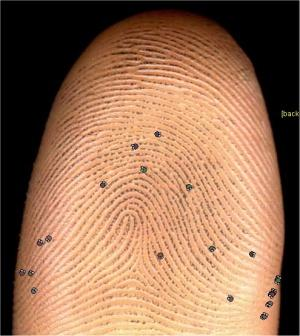
\includegraphics[width=7cm]{./4.jpg}
 \caption{Original Image}
\end{figure}
Orignal Image\\
\indent (300*336)pixels \\
\indent Size:47 kb\\[12pt]
\vskip-20pt
\begin{figure}[H]
 \centering
 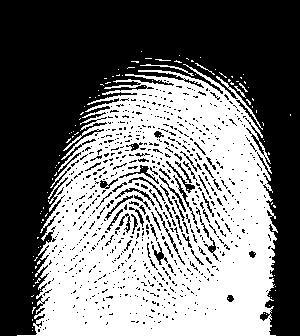
\includegraphics[width=7cm]{./5.jpg}
 \caption{Thresholded Image}
\end{figure}
\vskip5pt
After Otsu Thresholding\\
\indent (300*336)pixels\\
\indent Size:29.9 kb\\[12pt]
The advantage of Otsu method is that it produces more accurate results.\\[12pt]
The disadvantages of Otsu method is that it has lots of calculation involved in calculating weight,mean and variance.The histogram (and the image) are bimodal. The method assumes stationary statistics and cannot be modified to be locally adaptive. It assumes uniform illumination so the bimodalbrightness behavior arises from object appearance differences only.\\

\section{Thinning}

Fingerprint image thinning is a very important step in
fingerprint recognition algorithms. In this step the ridge
lines of the fingerprint image are transformed to a one-
pixel thickness. This process is fundamental for finger-
print recognition algorithms, as thinned images are
easier to process, and reduce operations processing time.\\[12pt]
As thinning does not change the structure of the finger-
print image and preserves the locations of the fingerprint
ridge and valley features, it makes easier to identify the
global and local features of the fingerprint image (such
as Core, Delta, Minutiae points) that are used for finger-
print classification, recognition and matching. \cite{pqr}





\begin{figure}[H]
 \centering
 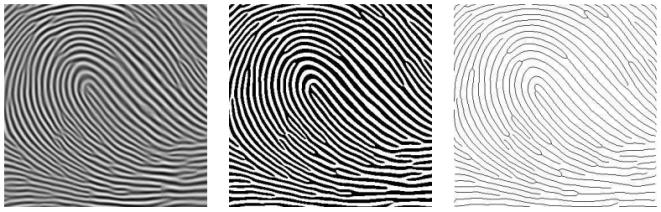
\includegraphics[width=12cm]{./8.jpg}
 \caption{From left to right: original fingerprint image, binarized image
and corresponding thinned image.}
\end{figure}


\section{Brightness}
Brightness can be calculated as:\\

Brightness=(0.2126*r) +( 0.7152*g)  +( 0.0722*b)

\section{Contrast}
(Maximum Brightness-Minimum Brightness) / (Maximum Brightness+Minimum Brightness)

\section{Scilab}
Scilab is an open source; cross-platform numerical computation package. It can be used for signal processing, image and video processing, numerical optimization and modeling and simulation of explicit and implicit systems. We made use of Scilab because it is an open source platform and provides good processing results.Image processing and enhancement needs packages like IPD and SIVP needed to installed separately. \cite{stu}


\chapter{Hardware}

It is the optical assembly mounted over the camera of the Aakash tablet.\\[12pt]
Apparatus used:\\[12pt]
\intend Black acrylic (3 mm thick)\\
Transparent acrylic (3 mm thick, 32.5mm x 35 mm)\\
PCB \\
LEDs (4 quantity, 3 mm thick)\\
Resistors (4 quantity, 220 ohms)\\
Wires\\
Driller\\
Soldering gun\\
Soldering wire\\
Hack saw\\
File\\
Polishing paper\\
Adapter (Output voltage: 5V DC)\\[12pt]
\intend Assembly consists of 3 parts-\\[12pt]
1. Clamp: To fix the assembly, with the tablet over the camera and also to hold the spacer.\\[12pt]
2. Spacer: To maintain a certain distance between the camera and fingerprint, such that a clear and consistent image is taken. \\[12pt]
3. Optical: To illuminate the finger, while fingerprint image has to be taken.\\[12pt]
\intend Clamp : It is made of black acrylic (opaque) which fits directly onto the camera of the Aakash tablet and there is also spacer holding capability of the clamp.\\[12pt]
Spacer : To get better focusing of the image, there should be a certain distance between the finger and the camera.  I have taken distance as 30 mm. I got this value by making cardboard prototypes of different heights of the spacer. Spacer is mounted on the clamp.\\[12pt]
Optical : This part is to actually implement the FTIR (frustrated total internal reflection) principle for fingerprint recognition. This consists of two parts-\\[12pt]
1. PCB : On this, leds are mounted just next to the acrylic plate on which fingerprint has to be kept. When we need to take the fingerprint image, LEDs glow and due to FTIR principle we get a fingerprint image which differentiates between the ridges and valleys of the finger.\\[12pt]
2. Lid : To cover the PCB so that outside light does not affect the fingerprint image.\\[12pt]
\vskip-25pt
\begin{figure}[H]
 \centering
 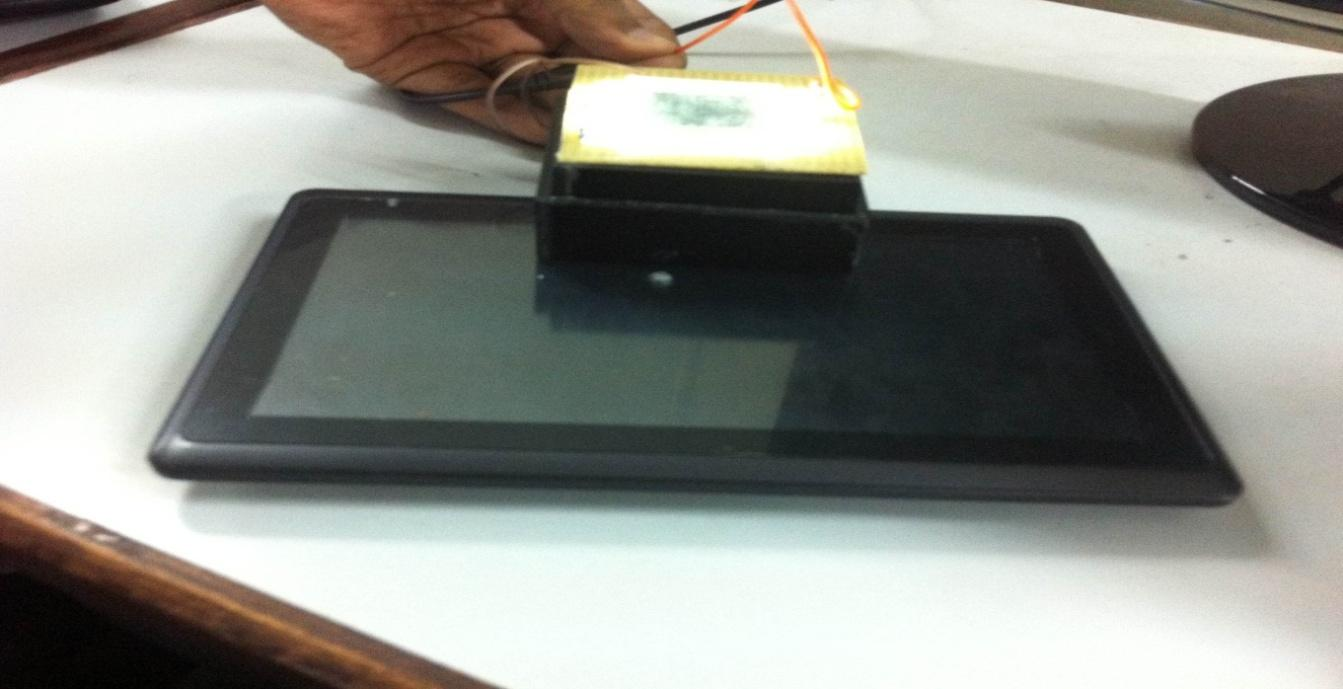
\includegraphics[width=15cm]{./6.jpg}
 \caption{Optical assembly attachment for Aakash tablet (Side view)}
\end{figure}
\begin{figure}[H]
 \centering
 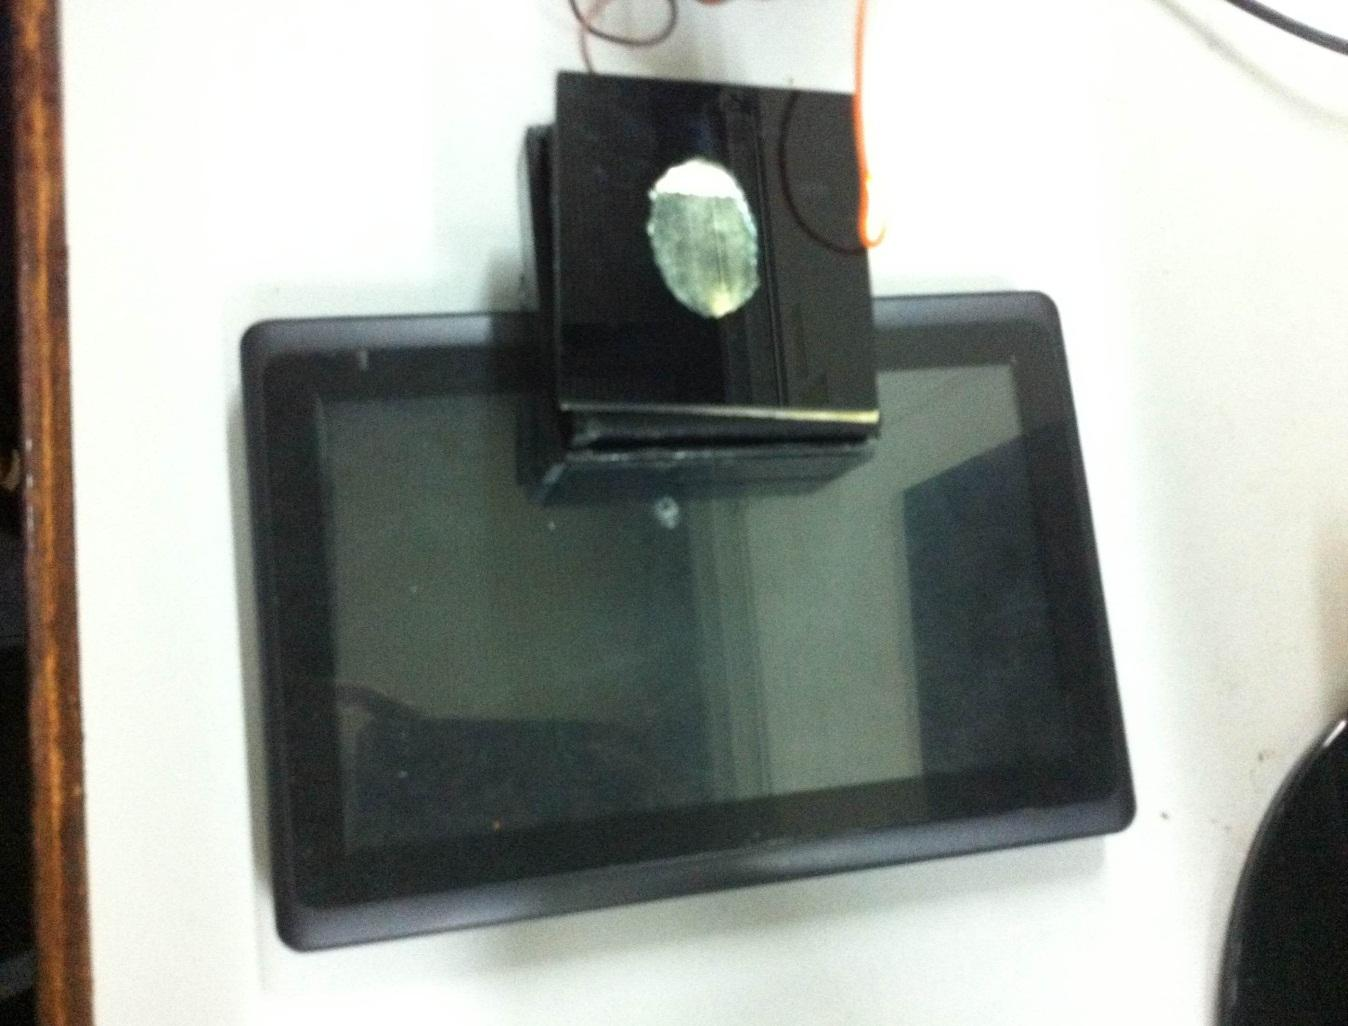
\includegraphics[width=12cm]{./88.jpg}
 \caption{Optical assembly attachment for Aakash tablet (Top View)}
\end{figure}

\chapter{Experimentation and Results}

Comparison of fingerprint image taken with optical assembly and without optical assembly:\\[12pt]

Without Optical assembly:\\[12pt]

\begin{figure}[H]
 \centering
 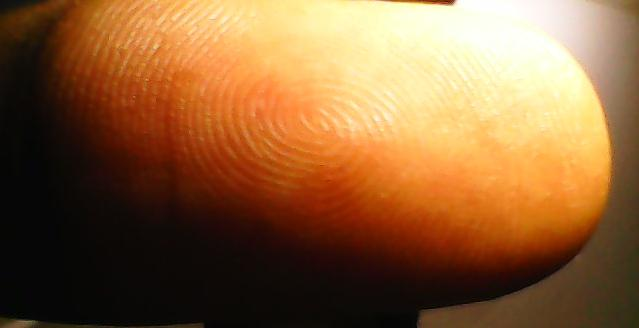
\includegraphics[width=10cm]{./10.jpg}
 \caption{Fingerprint Image}
\end{figure}


With Optical Assembly:\\[12pt]

\begin{figure}[H]
 \centering
 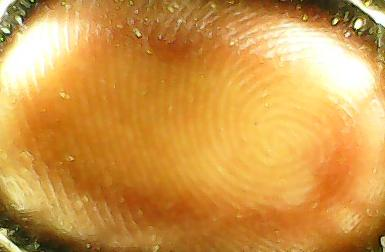
\includegraphics[width=8cm]{./11.jpg}
 \caption{Fingerprint Image}
\end{figure}


\section{Experiment 1-With NOKIA 5530}

\subsection{Input RGB Image}


\begin{figure}[H]
 \centering
 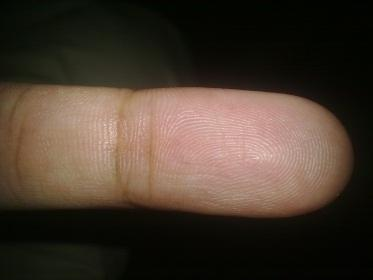
\includegraphics[width=8cm]{./12.jpg}
 \caption{Input Image}
\end{figure}

Specifications:\\[12pt]
Dimension:2048x1536\\
Size:233 KB\\
DPI:300\\
Filetype:.jpg\\
Colour Representation:RGB(values from 0 TO 255)\\
Exposure time:1/167 SECONDS\\
Focal Length:4 mm\\
Camera Specification:3.0 Megapixel\\[12pt]

Image Histogram:

\begin{figure}[H]
 \centering
 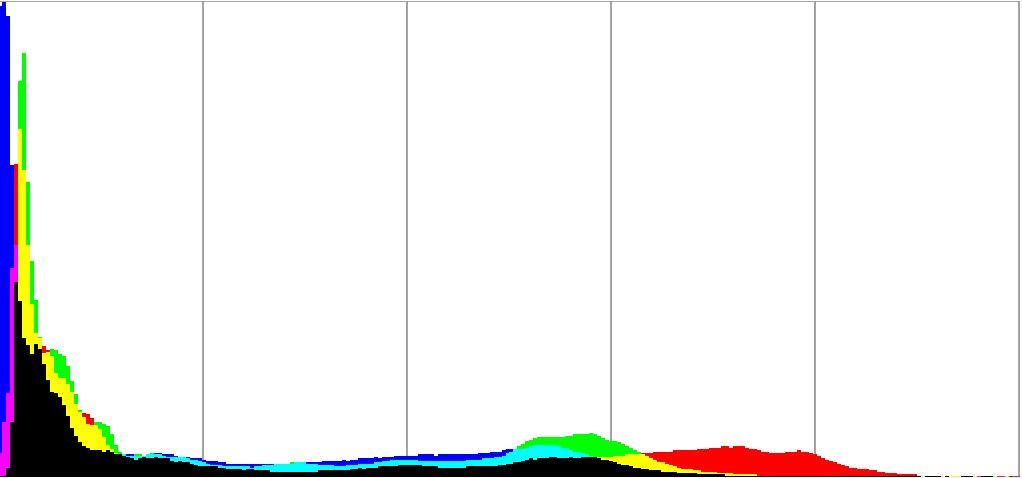
\includegraphics[width=8cm]{./13.jpg}
 \caption{Histogram}
\end{figure}
\vskip90pt
Brightness Histogram:

\begin{figure}[H]
 \centering
 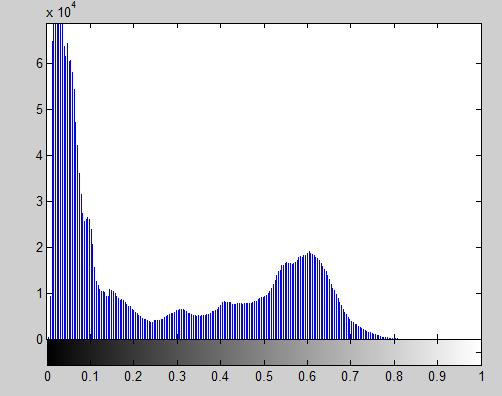
\includegraphics[width=7cm]{./14.jpg}
 \caption{Histogram}
\end{figure}
\newpage

\subsection{Cropped Image (Manual)}\\[12pt]


\begin{figure}[H]
 \centering
 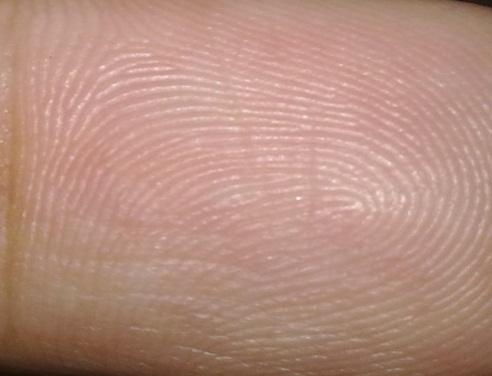
\includegraphics[width=6cm]{./15.jpg}
 \caption{Cropped Image}
\end{figure}

Specifications:\\[12pt]
Dimension:836x639\\
Size:64.2 KB\\
DPI:300\\
Filetype:.jpg\\
Contrast:0.8822\\[12pt]

Image Histogram:

\begin{figure}[H]
 \centering
 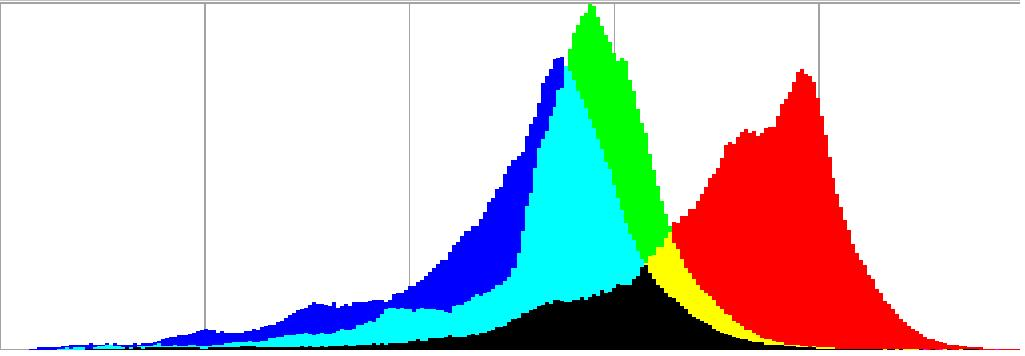
\includegraphics[width=8cm]{./16.jpg}
 \caption{Histogram}
\end{figure}

Brightness Histogram:

\begin{figure}[H]
 \centering
 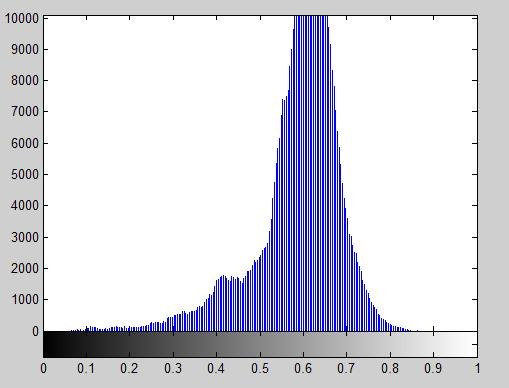
\includegraphics[width=8cm]{./17.jpg}
 \caption{Histogram}
\end{figure}
\newpage

\subsection{Image Grayscaling}\\[12pt]


\begin{figure}[H]
 \centering
 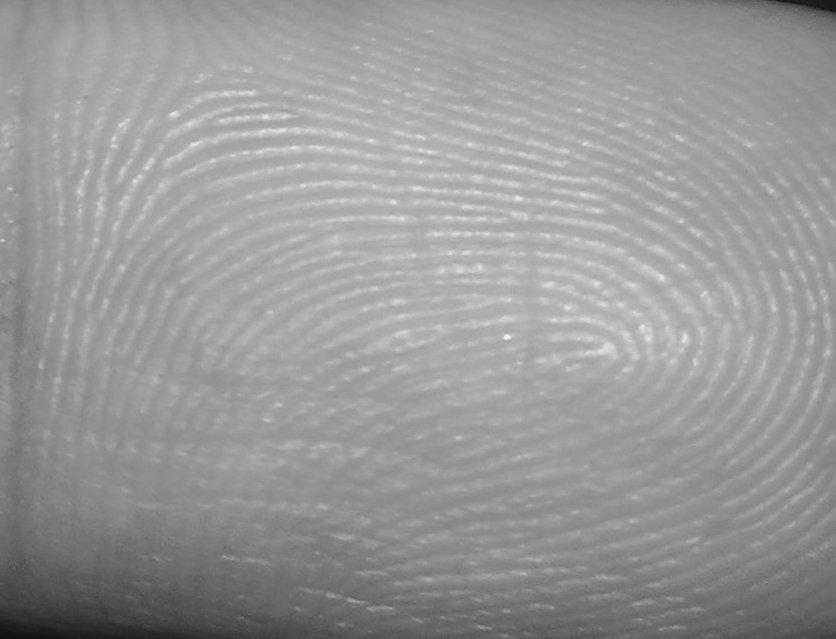
\includegraphics[width=6cm]{./18.jpg}
 \caption{Grayscaled Image}
\end{figure}

Specifications:\\[12pt]
Dimension:836x639\\
Size:46 KB\\
DPI:300\\
Filetype:.jpg\\[12pt]

Image Histogram:

\begin{figure}[H]
 \centering
 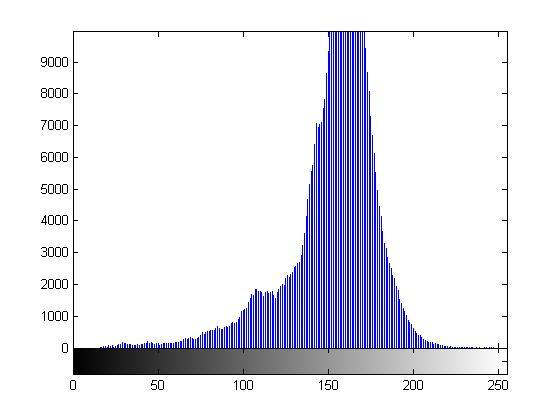
\includegraphics[width=8cm]{./19.jpg}
 \caption{Histogram}
\end{figure}
\newpage

\subsection{Image Resizing}\\[12pt]


\begin{figure}[H]
 \centering
 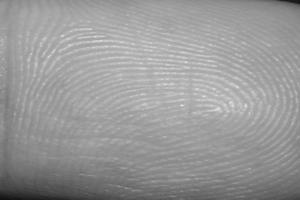
\includegraphics[width=6cm]{./20.jpg}
 \caption{Resized Image}
\end{figure}

Specifications:\\[12pt]
Dimension:300x200\\
Size:6.02 KB\\
DPI:300\\
Filetype:.jpg\\[12pt]

Image Histogram:

\begin{figure}[H]
 \centering
 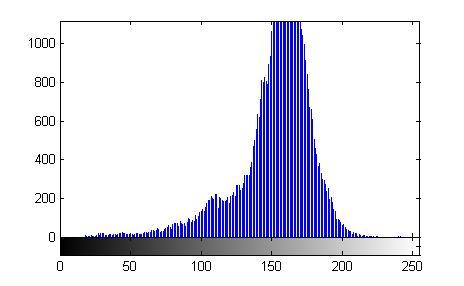
\includegraphics[width=8cm]{./21.jpg}
 \caption{Histogram}
\end{figure}
\newpage 

\subsection{Image Adaptive Histogram Equalization}\\[12pt]


\begin{figure}[H]
 \centering
 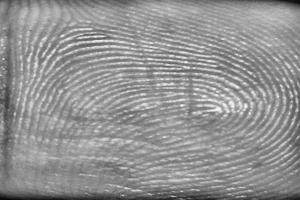
\includegraphics[width=6cm]{./22.jpg}
 \caption{Equalized Image}
\end{figure}

Specifications:\\[12pt]
Dimension:300x200\\
Size:12.1 KB\\
DPI:300\\
Filetype:.jpg\\[12pt]

Image Histogram:

\begin{figure}[H]
 \centering
 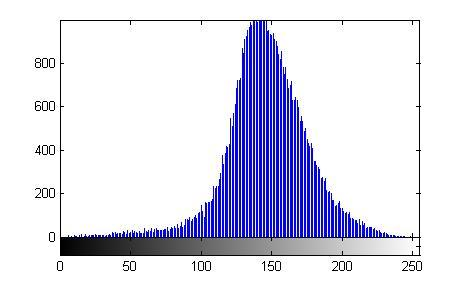
\includegraphics[width=8cm]{./23.jpg}
 \caption{Histogram}
\end{figure}
\newpage

\subsection{Image Sharpening}\\[12pt]


\begin{figure}[H]
 \centering
 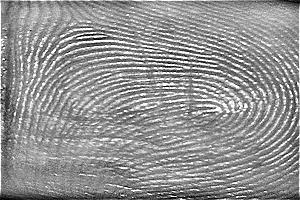
\includegraphics[width=6cm]{./24.jpg}
 \caption{Sharpened Image}
\end{figure}

Specifications:\\[12pt]
Dimension:300x200\\
Size:22.4 KB\\
DPI:300\\
Filetype:.jpg\\[12pt]

Image Histogram:

\begin{figure}[H]
 \centering
 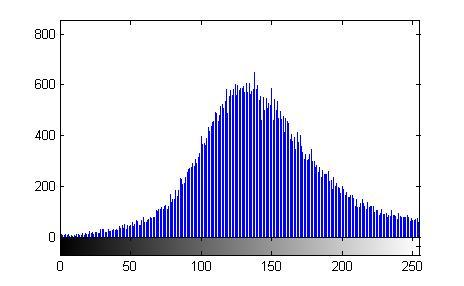
\includegraphics[width=8cm]{./25.jpg}
 \caption{Histogram}
\end{figure}
\newpage

\subsection{Image Thresholding}\\[12pt]


\begin{figure}[H]
 \centering
 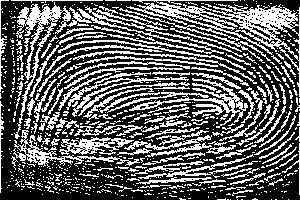
\includegraphics[width=6cm]{./26.jpg}
 \caption{Thresholded Image}
\end{figure}

Specifications:\\[12pt]
Dimension:300x200\\
Size:37.1 KB\\
DPI:300\\
Filetype:.jpg\\[12pt]

Image Histogram:

\begin{figure}[H]
 \centering
 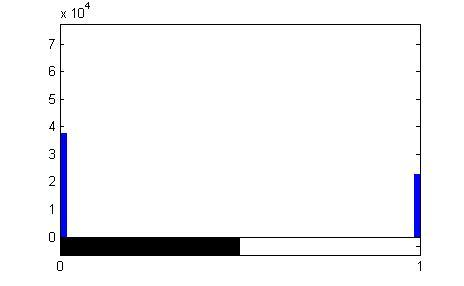
\includegraphics[width=8cm]{./27.jpg}
 \caption{Histogram}
\end{figure}
\newpage

\subsection{Image Thinning}\\[12pt]


\begin{figure}[H]
 \centering
 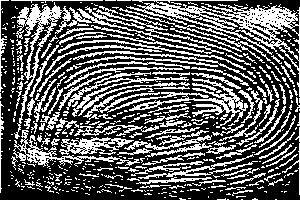
\includegraphics[width=6cm]{./28.jpg}
 \caption{Thinned Image}
\end{figure}

Specifications:\\[12pt]
Dimension:300x200\\
Size:36.6 KB\\
DPI:300\\
Filetype:.jpg\\[12pt]

Image Histogram:

\begin{figure}[H]
 \centering
 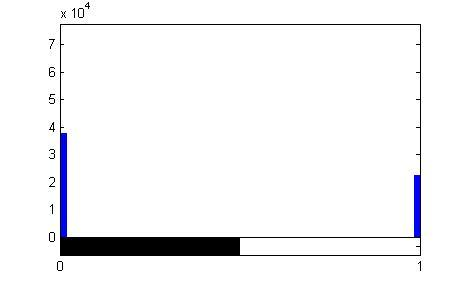
\includegraphics[width=8cm]{./29.jpg}
 \caption{Histogram}
\end{figure}
\newpage



\section{Experiment 2-With the Aakash Tablet}

\subsection{Input RGB Image}\\[12pt]


\begin{figure}[H]
 \centering
 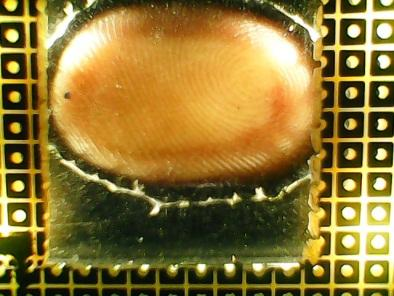
\includegraphics[width=8cm]{./30.jpg}
 \caption{Input Image.}
\end{figure}

Specifications:\\[12pt]
Dimension:640x480\\
Size:159 KB\\
DPI:96\\
Filetype:.jpg\\
Colour Representation:RGB(values from 0 TO 255)\\
Camera Maker: MID 001\\
Focal Length:3 mm\\
Camera Specification:0.3 MEGAPIXELS VGA\\[12pt]

Image Histogram:

\begin{figure}[H]
 \centering
 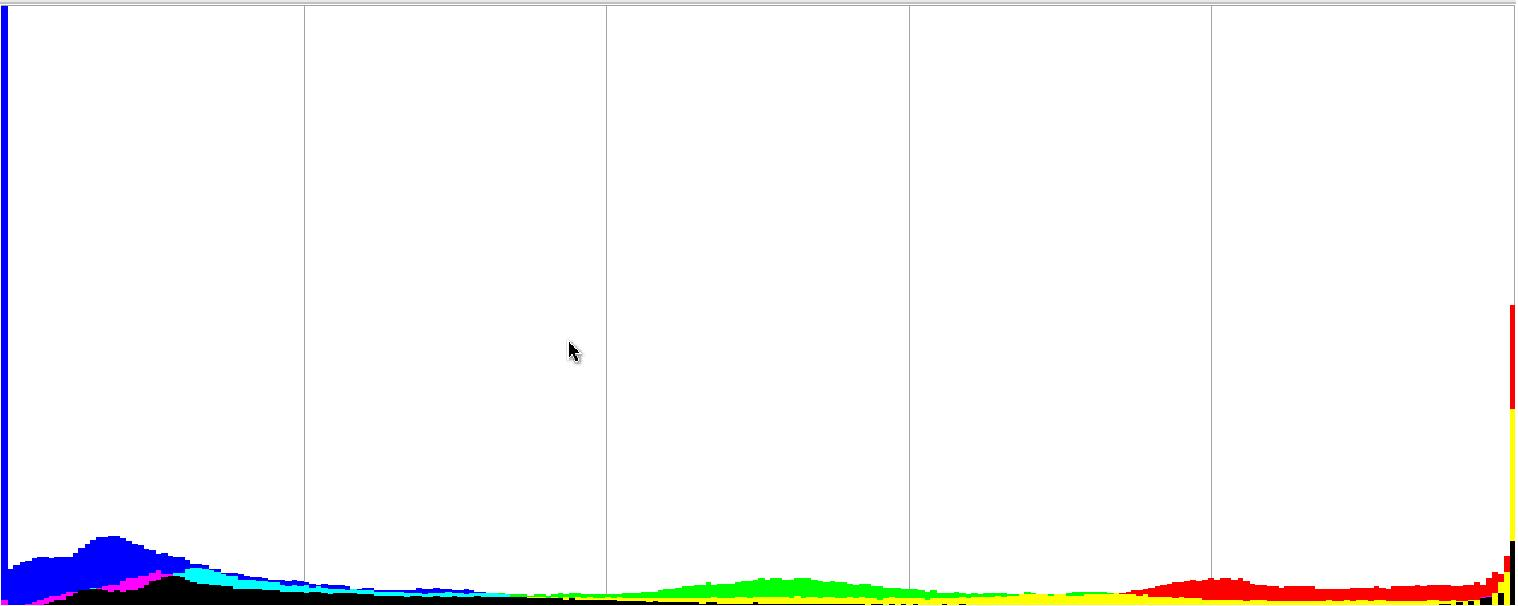
\includegraphics[width=8cm]{./31.jpg}
 \caption{Histogram.}
\end{figure}

\newpage

\subsection{Cropped Image (Manual)}\\[12pt]


\begin{figure}[H]
 \centering
 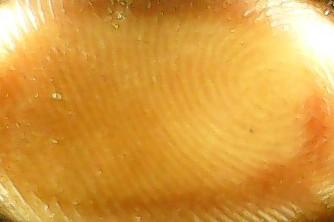
\includegraphics[width=6cm]{./32.jpg}
 \caption{Cropped Image.}
\end{figure}

Specifications:\\[12pt]
Dimension:334x222\\
Size:16.1 KB\\
DPI:96\\
Filetype:.jpg\\
Contrast:0.7853\\[12pt]

Image Histogram:

\begin{figure}[H]
 \centering
 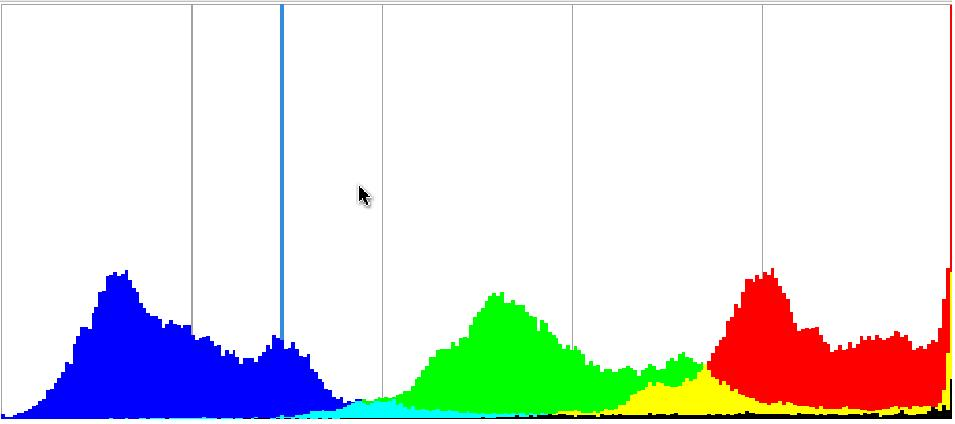
\includegraphics[width=8cm]{./33.jpg}
 \caption{Histogram.}
\end{figure}

\newpage 

\subsection{Image Grayscaling}\\[12pt]


\begin{figure}[H]
 \centering
 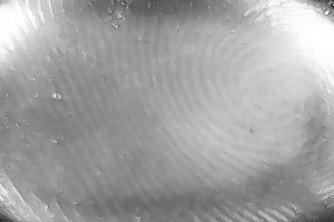
\includegraphics[width=6cm]{./34.jpg}
 \caption{Grayscaled Image.}
\end{figure}

Specifications:\\[12pt]
Dimension:334x222\\
Size:6.66KB\\
DPI:96\\
Filetype:.jpg\\[12pt]

Image Histogram:

\begin{figure}[H]
 \centering
 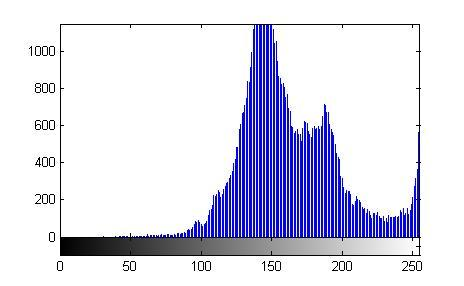
\includegraphics[width=8cm]{./35.jpg}
 \caption{Histogram.}
\end{figure}
\newpage

\subsection{Image Resizing}\\[12pt]


\begin{figure}[H]
 \centering
 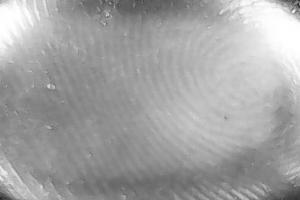
\includegraphics[width=6cm]{./36.jpg}
 \caption{Resized Image.}
\end{figure}

Specifications:\\[12pt]
Dimension:300x200\\
Size:5.77 KB\\
DPI:96\\
Filetype:.jpg\\[12pt]

Image Histogram:

\begin{figure}[H]
 \centering
 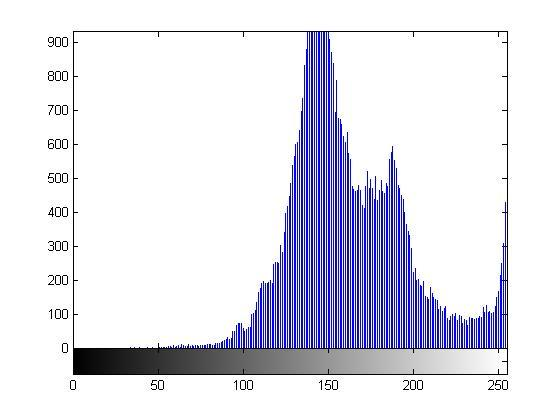
\includegraphics[width=8cm]{./37.jpg}
 \caption{Histogram.}
\end{figure}
\newpage

\subsection{Image Adaptive Histogram Equalization}\\[12pt]


\begin{figure}[H]
 \centering
 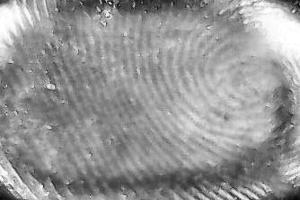
\includegraphics[width=6cm]{./38.jpg}
 \caption{Equalized Image.}
\end{figure}

Specifications:\\[12pt]
Dimension:300x200\\
Size:10.8 KB\\
DPI:96\\
Filetype:.jpg\\[12pt]

Image Histogram:

\begin{figure}[H]
 \centering
 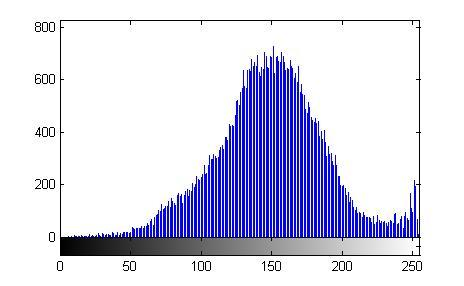
\includegraphics[width=8cm]{./39.jpg}
 \caption{Histogram.}
\end{figure}
\newpage

\subsection{Image Sharpening}\\[12pt]


\begin{figure}[H]
 \centering
 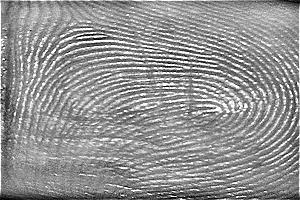
\includegraphics[width=6cm]{./24.jpg}
 \caption{Sharpened Image.}
\end{figure}

Specifications:\\[12pt]
Dimension:300x200\\
Size:19.2 KB\\
DPI:96\\
Filetype:.jpg\\[12pt]

Image Histogram:

\begin{figure}[H]
 \centering
 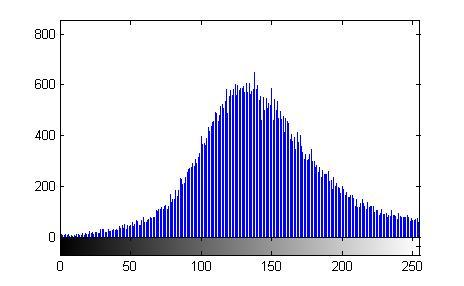
\includegraphics[width=8cm]{./25.jpg}
 \caption{Histogram.}
\end{figure}
\newpage

\subsection{Image Thresholding}\\[12pt]


\begin{figure}[H]
 \centering
 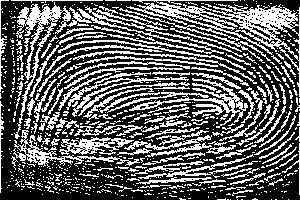
\includegraphics[width=6cm]{./26.jpg}
 \caption{Thresholded Image.}
\end{figure}

Specifications:\\[12pt]
Dimension:300x200\\
Size:31.9 KB\\
DPI:96\\
Filetype:.jpg\\[12pt]

Image Histogram:

\begin{figure}[H]
 \centering
 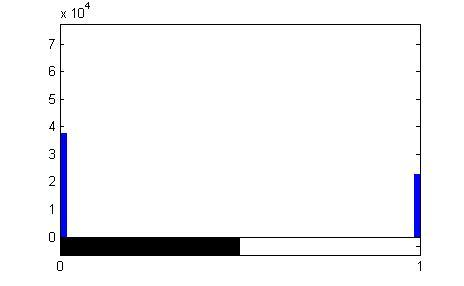
\includegraphics[width=8cm]{./27.jpg}
 \caption{Histogram.}
\end{figure}
\newpage

\subsection{Image Thinning}\\[12pt]


\begin{figure}[H]
 \centering
 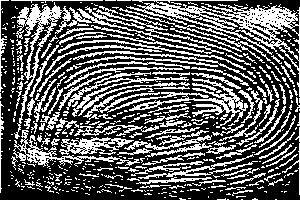
\includegraphics[width=6cm]{./28.jpg}
 \caption{Thinned Image.}
\end{figure}

Specifications:\\[12pt]
Dimension:300x200\\
Size:31.0 KB\\
DPI:96\\
Filetype:.jpg\\[12pt]

Image Histogram:

\begin{figure}[H]
 \centering
 \includegraphics[width=8cm]{./29.jpg}
 \caption{Histogram.}
\end{figure}
\newpage

\section{Experimental Results With Different Number of Leds ON}\\[12pt]

\subsection{With all LEDs on}\\[12pt]

\subsubsection{Cropped Image (Manual)}\\[12pt]

\begin{figure}[H]
 \centering
 \includegraphics[width=8cm]{./61.jpg}
 \caption{Histogram.}
\end{figure}


Specifications:\\[12pt]
Dimensions:386 x 398\\
Size:219 KB\\
DPI:96\\
File Type:.jpg\\[12pt]


Image Histogram:

\begin{figure}[H]
 \centering
 \includegraphics[width=8cm]{./62.jpg}
 \caption{Histogram.}
\end{figure}

\newpage

\subsection{With 3 Leds on}\\[12pt]

\subsubsection{Cropped Image (Manual)}\\[12pt]

\begin{figure}[H]
 \centering
 \includegraphics[width=8cm]{./63.jpg}
 \caption{Histogram.}
\end{figure}

Specifications:\\[12pt]
Dimensions:447x 315\\
Size:29 KB\\
DPI:96\\
File Type:.jpg\\[12pt]

Image Histogram:

\begin{figure}[H]
 \centering
 \includegraphics[width=8cm]{./64.jpg}
 \caption{Histogram.}
\end{figure}

\newpage

\subsection{With 2 Leds(adjacent) on}\\[12pt]

\subsubsection{Cropped Image (Manual)}\\[12pt]

\begin{figure}[H]
 \centering
 \includegraphics[width=8cm]{./65.jpg}
 \caption{Histogram.}
\end{figure}

Specifications:\\[12pt]
Dimensions:452x323\\
Size:30.4 KB\\
DPI:96\\
File type:.jpg\\[12pt]

Image Histogram:

\begin{figure}[H]
 \centering
 \includegraphics[width=8cm]{./66.jpg}
 \caption{Histogram.}
\end{figure}

\newpage

\subsection{With 2 Leds(diagonal) on}\\[12pt]

\subsubsection{Cropped Image (Manual)}\\[12pt]

\begin{figure}[H]
 \centering
 \includegraphics[width=8cm]{./67.jpg}
 \caption{Histogram.}
\end{figure}

Specifications:\\[12pt]
Dimensions:427x291\\
Size:24.3 KB\\
DPI:96\\
File type:.jpg\\[12pt]

Image Histogram:

\begin{figure}[H]
 \centering
 \includegraphics[width=8cm]{./68.jpg}
 \caption{Histogram.}
\end{figure}

\newpage

\subsection{With 1 Led on} \\[12pt]

\subsubsection{Cropped Image (Manual)}\\[12pt]

\begin{figure}[H]
 \centering
 \includegraphics[width=8cm]{./69.jpg}
 \caption{Histogram.}
\end{figure}

Specifications:\\[12pt]
Dimensions:449x310\\
Size:27.8 KB\\
DPI:96\\
File type:.jpg\\[12pt]

Image Histogram:

\begin{figure}[H]
 \centering
 \includegraphics[width=8cm]{./70.jpg}
 \caption{Histogram.}
\end{figure}



\chapter{Conclusion and Future Scope}

In today's world, it is important to be secure from every possible area which has threads of being attacked. With emerging technology the security can be much effectively used.

The reliability of any automatic fingerprint system strongly relies on the precision obtained in the minutia extraction process. A number of factors are detrimental to the correct location of minutia. Among them, poor image quality is the most serious one. In this project, wehave combined many methods to build a minutia extractor and a minutia matcher. The following concepts have been used- segmentation using Morphological operations, minutia marking byespecially considering the triple branch counting, minutia unification by decomposing a branch into three terminations and matching in the unified x-y coordinate system after a 2-step transformation in order to increase the precision of the minutia localization process and elimination of spurious minutia with higher accuracy.\\[12pt]

The proposed alignment-based elastic matching algorithm is capable of finding the correspondences between minutiae without resorting to exhaustive research.\\[12pt]

There is a scope of further improvement in terms of efficiency and accuracy which can be achieved by improving the accuracy of the optical assembly by testing with IR and SMD LEDs so as to capture better image or by improving the image enhancement techniques so that the input image to the thinning stage could be made better which could improve the future stages and the final outcome.\\[12pt]



\bibliographystyle{ieeetr}
\bibliography{biblio}

\end{document}